% !TEX root = MasterPaper.tex
\chapter{先行研究}
\thispagestyle{fancy} % このページのみ
\lhead{}
\chead{}
\rhead{}
\lfoot{} 
\cfoot{\thepage}  
\rfoot{}
%

\section{遺伝的アルゴリズム}
\label{sec2.1}

\subsection{遺伝的アルゴリズムの概要}
\label{sec2.1.1}

GAとは選択淘汰や突然変異など生物進化の仕組みを模範した最適化アルゴリズムである\cite{GA}.GAの基本的な枠組みは非常に簡単で,与えられた最適化問題の評価関数に対し,いくつかの乱数と単純な記号処理を用いるだけで,比較的少ない計算量で(準)最適解を効率よく求めることができる\cite{GA}.

GAのフローチャートを図\ref{遺伝的アルゴリズムのフローチャート}に示す.GAでは生成した遺伝子列に対して,選択,交叉,突然変異といった生物進化の仕組みを模した処理を行う.問題の解候補を生物集団の各個体と呼び,各個体のパラメータを遺伝子と呼ぶ.

以下に図\ref{遺伝的アルゴリズムのフローチャート}の具体的な流れについて述べる.


\begin{description}
\item[ (1) ]遺伝子型の決定

GAの対象となる問題を遺伝子列にコーディングする.

\item[ (2) ]初期遺伝子集団の決定

(1)で決められた遺伝子型で要素の異なるの個体をランダムに発生させる.

\item[ (3) ]適応度評価

生成された遺伝子集団に対して評価し,各個体の適応度をあらかじめ定められた計算方法と評価結果に基づいて算出する.

\item[ (4) ]選択処理

遺伝子集団中における各個体の適応度に基づいて,交叉処理を行う個体を選択する.

\item[ (5) ]交叉処理

(4)で選択された2つの個体間で遺伝子を組み替えて新しい個体を発生させる.

\item[ (6) ]突然変異処理

個体の遺伝子を特定の確率で一部だけ,強制的に変化させる.

\item[ (7) ]終了条件(遺伝子集団の評価)

生成された次世代の遺伝子集団が,GA処理を終了するための評価基準を満足しているかどうかを確認する.
\end{description}

\begin{figure}[p]
\begin{center}

\vspace{1.5cm}
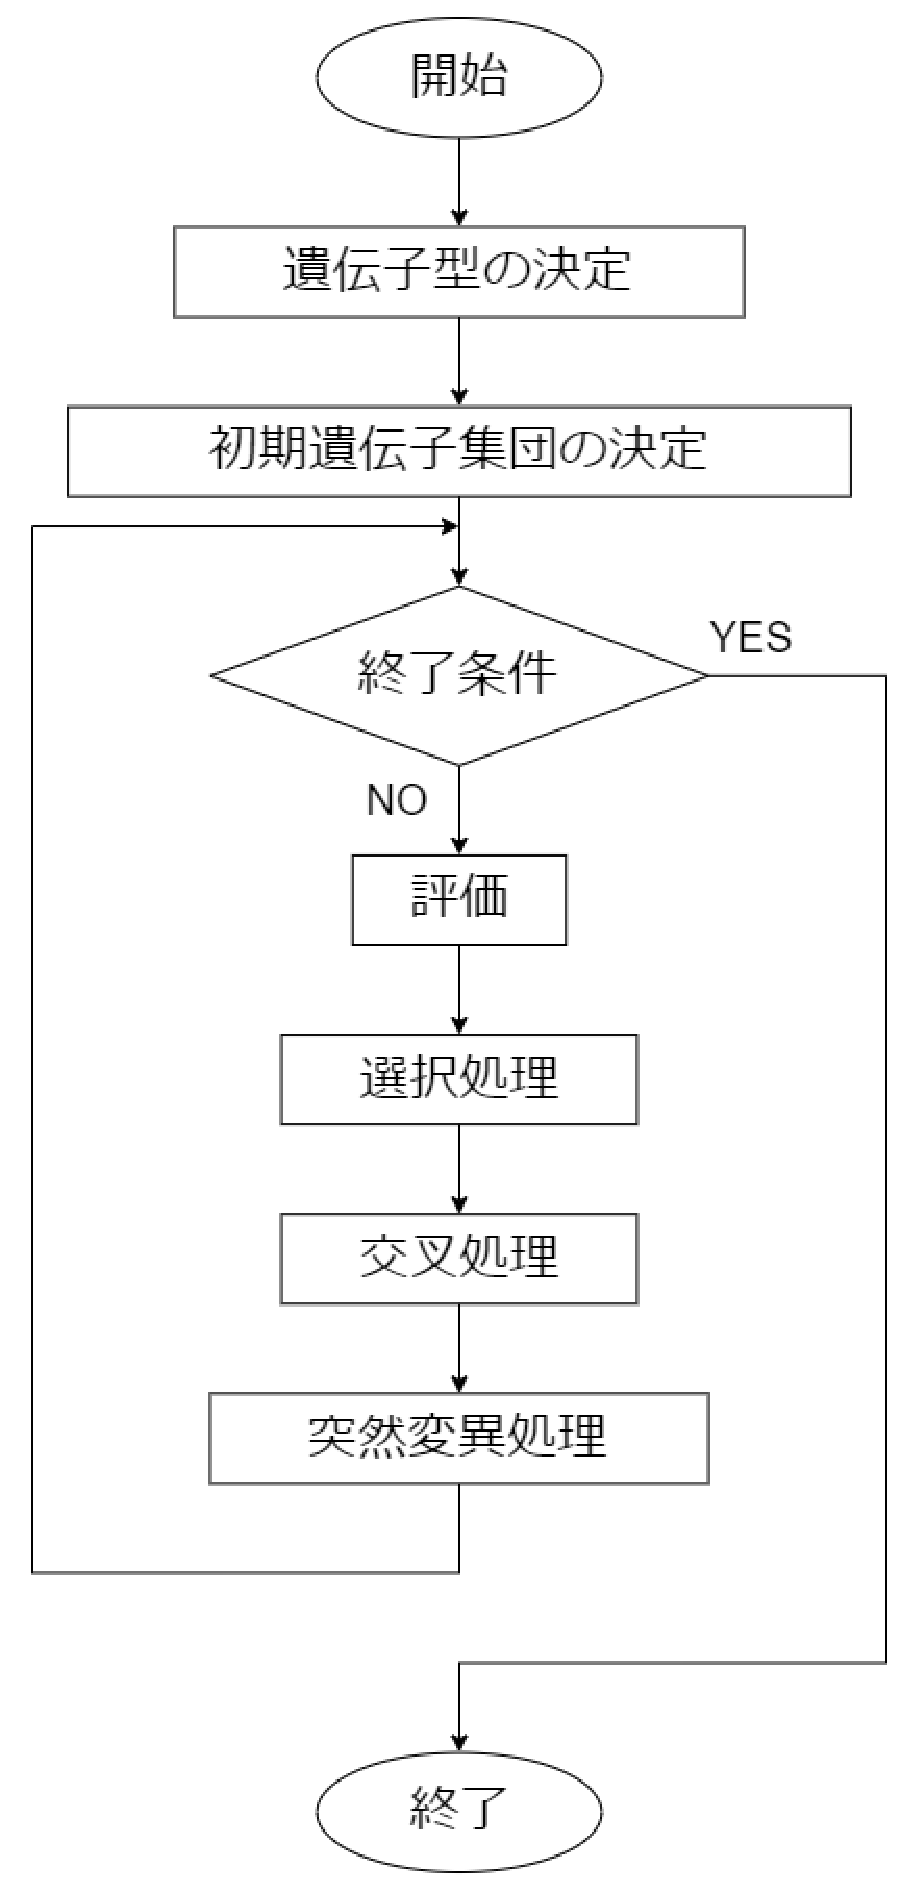
\includegraphics[scale=0.6]{figure/chapter2/GAflow.eps}
\caption{GAのフローチャート}
\label{遺伝的アルゴリズムのフローチャート}

\end{center}
\end{figure}

\clearpage


\subsection{各個体の評価処理}
\label{sec2.1.2}
  
各個体の評価処理は,あらかじめ定めた適応度により,各個体の適応度を求める操作である.本処理は遺伝子型と設定されている記号列を実際の評価型にデコーディングして,その表現型と設定されている環境との適応を判定することによって行われる.しかし,個体間で適応度の差が激しい場合,選択処理時に適応度の高い個体が選ばれる確率が非常に高くなる.その個体の遺伝子が集団内に爆発的に増加することで,探索がかなり早い段階で収束してしまい,初期収束が起きる可能性が非常に高くなる.そこで適応度の差を拡大,あるいは縮小するためにスケーリング関数を用いて,適切な選択を実現させる.スケーリング関数の例を表2.1に示す.表2.1において$f$は元の適応度,$f'$は新たな適応度である.べき乗スケーリングにおいて,$k$はスケーリング指数と呼ばれる.また,シグマ切断の関数において,$\sigma$は適応度の標準偏差,$\bar{f}$は適応度の平均値である.



\begin{table}[!ht]
\caption{スケーリング関数の例}
\label{tb:sk}
\begin{center}
\begin{tabular}{|c||c|}\hline
スケーリング & 関数 \\ \hline
線形スケーリング & $f'=af+b$ \\ \hline
べき乗スケーリング & $f'=f^{k}$ \\ \hline
シグマ切断 & $f'=f-( \bar{f} - c \times \sigma )$ \\ \hline
\end{tabular}
\end{center}
\end{table}

\newpage


\subsection{選択処理}
\label{sec2.1.3}

各個体の選択処理は,集団内での適応度の分布にしたがって,交叉を行う個体を決定する操作である.以下に,基本的な選択処理方法である適応度比例方式とエリート保存方式について述べる.

\begin{description}
\item[ (1) ]適応度比例方式

適応度比例方式はルーレット選択方式とも呼ばれ,適応度に比例した確率で親となる個体を選択する方法である.適応度比例方式の最も簡単な実現方法は,適応度に比例した領域をもつルーレットを回し,ルーレットの玉が入った領域の個体を選び出すというものである.
式(\ref{eq:2.1})に重み付けルーレット方式の式を示す.



\begin{equation}
\vspace{1.0cm}
{p_i}=\frac{f_i}{\displaystyle\sum_{i=1}^{n}f_i}
\label{eq:2.1}
\vspace{-0.5cm}
\end{equation}
式(\ref{eq:2.1})において,$p_i$は$i$番目の個体が親として選択される確率,$f_i$は$i$番目の個体適応度,$n$は個体数である.

\item[ (2) ]エリート保存方式

エリート保存方式は,個体の中で最も適応度の高い個体をそのまま次世代に残す方法である.その時点で最も適応度の高い個体は交叉や突然変異により破壊されない利点がある.ただし,適応度の高い個体が集団内で急速に増加する可能性が高いため,局所最適解に陥る危険性がある.そのため,一般的には他の選択方法と組み合わせて用いられる.

\end{description}

\newpage

\subsection{交叉処理}
\label{sec2.1.4}

交叉処理は,2つの染色体間で遺伝子を組み替えて,新たな個体を発生させる操作である.交叉処理は性質上,GAで最も重要な処理である.
交叉処理で用いられる基本的な手法である一点交叉,複数点交叉,一様交叉についての例を図\ref{tb:cross}に示す.



\begin{description}
\item[ (1) ]一点交叉

図\ref{一点交叉}に示すように,遺伝子に交叉位置をランダムで一点決定する.交叉位置で,親1と親2の遺伝子を入れ替え,子1と子2を発生させる.


\item[ (2) ]複数点交叉

図\ref{複数点交叉}に示すように,遺伝子に複数の交叉位置を作る.交叉位置ごとに親1と親2の遺伝子を入れ替え,子1と子2を発生させる.

\item[ (3) ]一様交叉

図に\ref{一様交叉}示すように,マスクパターンをランダムに生成する.そして,2つの親個体に対し,そのマスクのビットが0であるなら親1を,1であるなら親2の遺伝子をコピーして子1を発生させる.同時に逆のコピーを行い,子2を発生させる.

\end{description}

\newpage

\begin{figure}[p]
\begin{center}


\subfigure[一点交叉]{
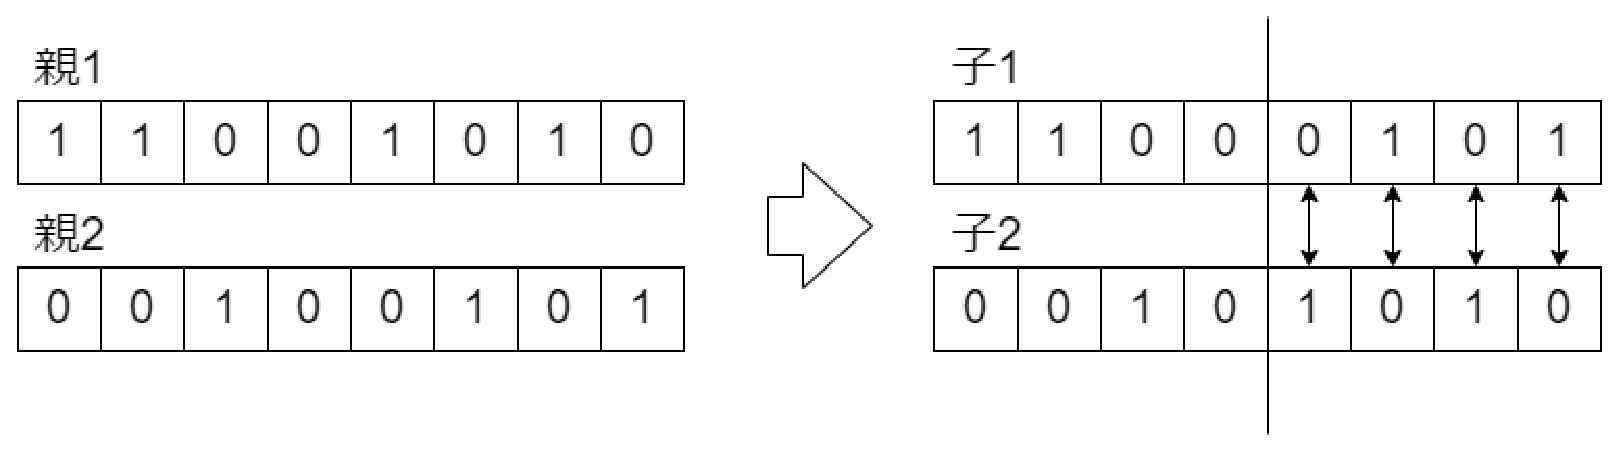
\includegraphics[width=15cm]{figure/chapter2/crossover_1.eps}
\label{一点交叉}}

\subfigure[複数点交叉]{
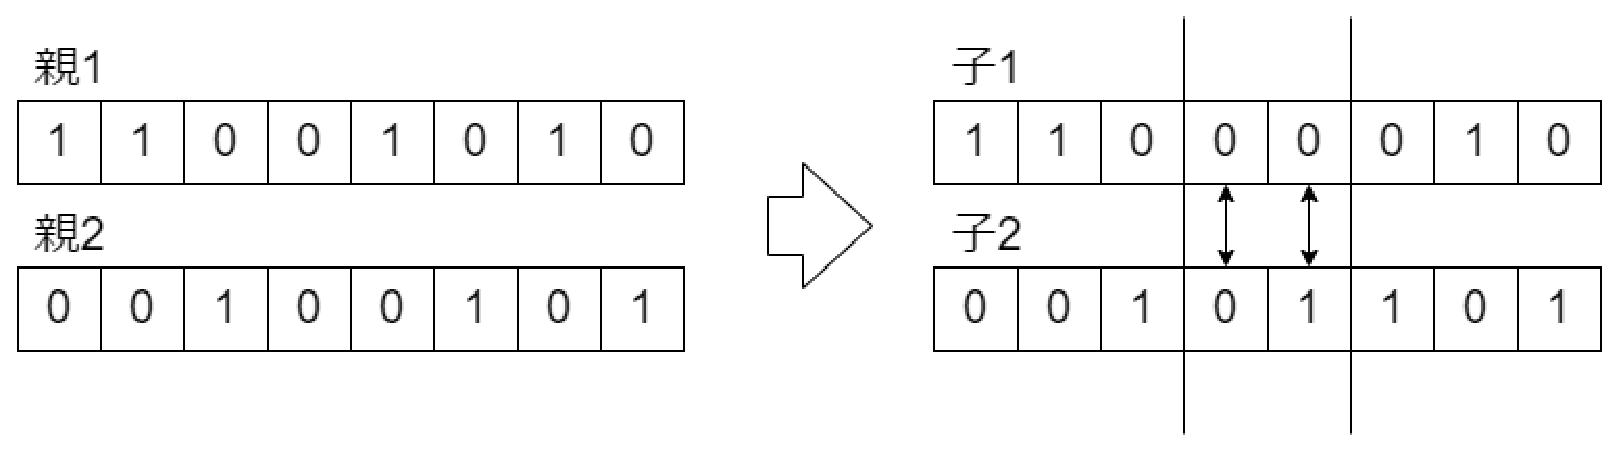
\includegraphics[width=15cm]{figure/chapter2/crossover_2.eps}
\label{複数点交叉}}

\subfigure[一様交叉]{
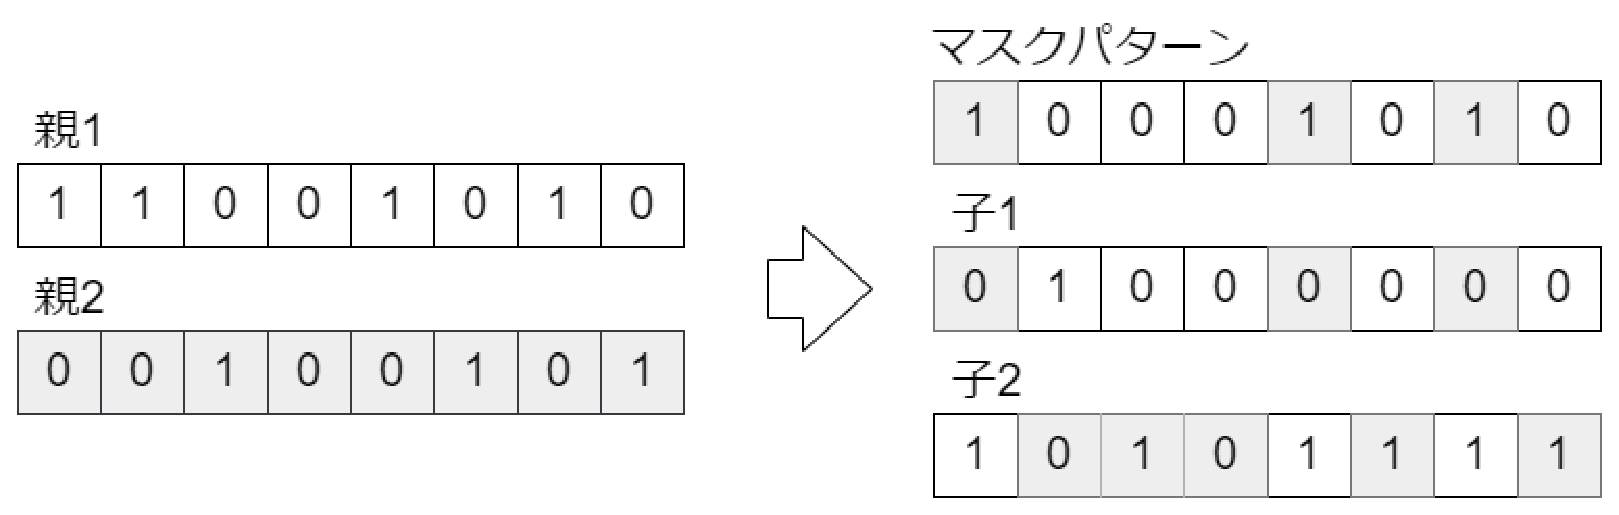
\includegraphics[width=15cm]{figure/chapter2/crossover_3.eps}
\label{一様交叉}}

\caption{交叉処理}
\label{tb:cross}


\end{center}

\end{figure}



\clearpage



\subsection{突然変異処理}
\label{sec2.1.5}

突然変異処理は,遺伝子のある部分を特定の確率で強制的に変化させる操作である.この操作により遺伝子集団に多様性を生み出し,より良い解を持つ個体の発生を促す.交叉処理で用いられる基本的な手法である転座方式,逆位方式について図\ref{fig:2.3}に示す.

\begin{description}

\item[ (1) ]転座方式

図\ref{転座方式}に転座方式を示す.転座方式は,遺伝子の一部が同じ遺伝子の他の部分,または他の遺伝子上に位置を移す処理である.

\item[ (2) ]逆位方式


図\ref{逆位方式}に逆位方式を示す.逆位方式は,部分的に遺伝子の配列順序を入れ替える処理である.


\end{description}

\begin{figure}[hbt]
\centering
\subfigure[転座方式]{
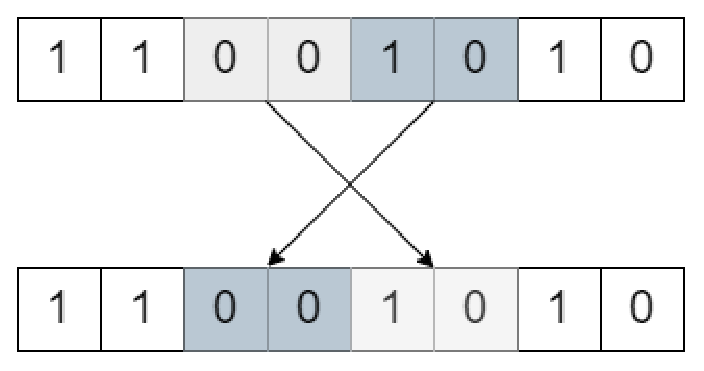
\includegraphics[scale=0.8]{figure/chapter2/mutation_1.eps}
\label{転座方式}}


\subfigure[逆位方式]{
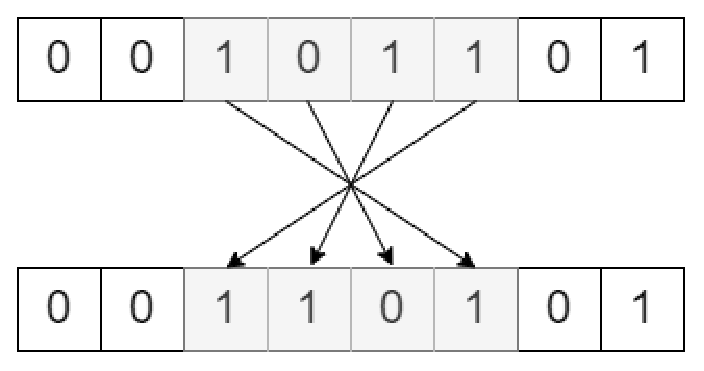
\includegraphics[scale=0.8]{figure/chapter2/mutation_2.eps}
\label{逆位方式}}


\caption{突然変異処理}
\label{fig:2.3}
\end{figure}


\newpage

\section{対話型進化計算}
\label{sec2.2}

\subsection{対話型進化計算の概要}
\label{sec2.2.1}

感性情報を扱う以前では,情報処理におけるシステムの最適化とは,望ましいシステム出力が得られるようにシステムパラメータを調節することであった.ほとんどの場合,望ましいシステム出力とは数値的ゴールのことを指し,誤差最小化規範などを代表とする各種最適化手法が開発されてきた\cite{GA2}.

しかし近年では,情報処理におけるシステムの最適化の対象は,感性情報にまで拡大している.ユーザが好む音楽や画像などが望ましい出力の場合は,個人の主観的な直感を扱う感性による評価しかできないという問題がある.このようなシステム最適化において,従来とは異なる最適化手法が必要となる.その方法の一つとして,ユーザの評価系の代替モデルを作成し,従来の最適化システムに組み込むことで数値的に求めることが挙げられる.しかし,個人の好みに対応できる正確な代替モデルの構築は非常に難しい.

そこで,ユーザ自身を最適化系に組み込み,ユーザ本人の評価に基づいてコンピュータに最適化させる方法が考えられる.このようにユーザとコンピュータとの相互作用により,ユーザの主観的評価に基づいて最適化する手法のうち,ECを用いる手法をIECと呼ぶ\cite{IEC}.IEC システムにおいては,評価関数が解候補の適応度評価を行うのではなく,ユーザがシステムの出力を見たり聞いたりして直感的な主観で評価する.そして,その評価値に基づいた結果を用いて,ユーザにとって望ましいと予想される出力が得られるようにECを行い,システムを最適化する.IECは人間の主観的評価に基づく最適化手法であるため,感性を具現化する技術といえる.

代表的なEC 技術として,GA,タブーサーチ法(Taboo Serch: TS),遺伝的プログラミング (Genetic Programming: GP),進化戦略 (Evolution Strategy: ES),進化的プログラミング (Evolutionary Programming: EP),粒子群最適化 (Particle Swarm Optimization: PSO) などがある.
    
\subsection{対話型遺伝的アルゴリズム}
\label{sec2.2.2}

本研究では,GAにおける評価系に人の感性を組み込んだ手法であるIGAを用いる.
IGAは,GA処理における解候補評価をユーザが自らの感性に基づいて行い,解候補を最適化する手法である.

IGAの基本的な処理の流れを図\ref{対話型遺伝的アルゴリズムのフローチャート}に示す.まず初期解候補群を生成する.次に,解候補をユーザに提示し,解候補を主観的に評価してもらう.ユーザによる評価が終了すると,ユーザによって与えられた各解候補の評価値をもとに選択・交叉・突然変異等の処理が行う.そして,新たな解候補を生成し,再びユーザに提示する.このような処理を繰り返し,ユーザの感性に合う解候補を生成する.

IGAは,ユーザ評価を取り入れた進化計算手法であるIECにおいてGAの進化計算アルゴリズムを適応させた手法である.すなわち,IGAとは通常のGAにおいて適応度を決定する処理をユーザが行う手法である.ユーザの主観的評価が適応度に反映されるため,IGAは特にユーザの感覚的,直観的な評価が必要とされる問題の解決に多く用いられる.
\begin{figure}[p]
\begin{center}

\vspace{1.5cm}
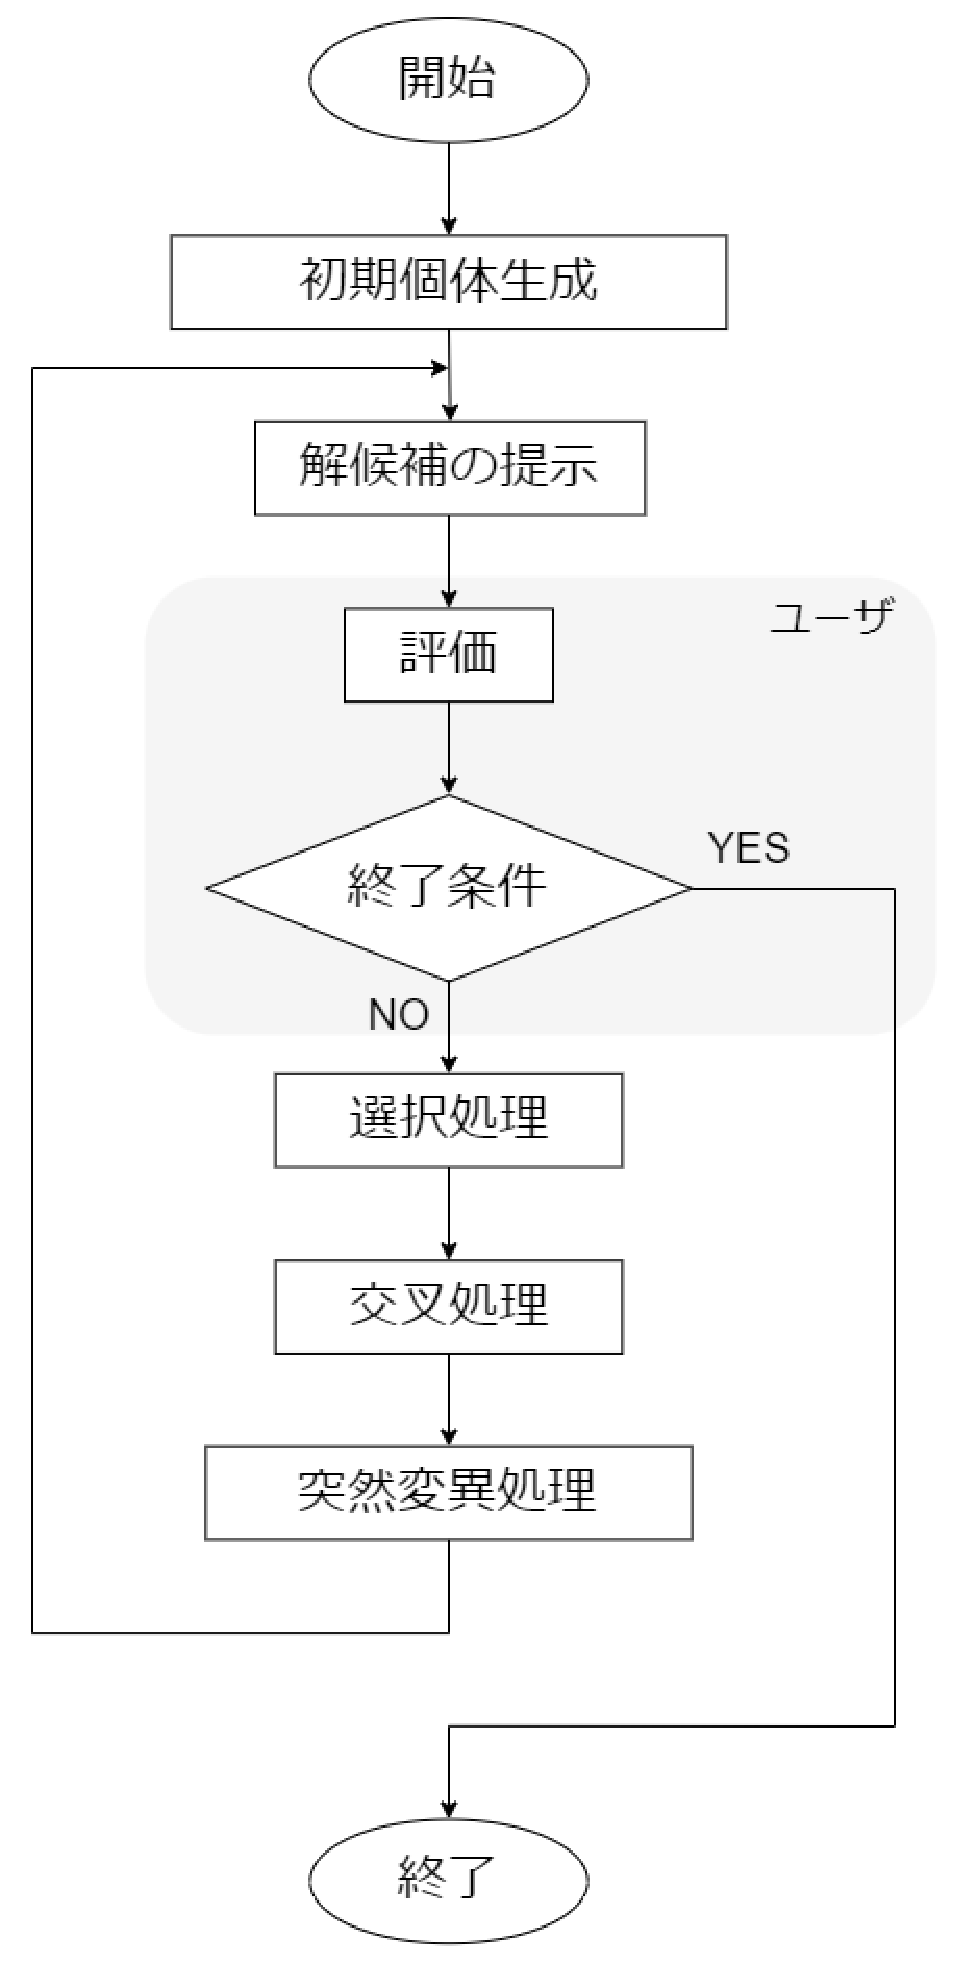
\includegraphics[scale=0.6]{figure/chapter2/IGAflow.eps}
\caption{IGAのフローチャート}
\label{対話型遺伝的アルゴリズムのフローチャート}

\end{center}
\end{figure}



\newpage

\section{感性とロボット}
\label{sec2.3}

\subsection{ロボットの進化}
\label{sec2.3.1}
人間の代わりに工場などで過酷な作業を行う産業用ロボットは.1960年代に開発が進み,1980年代から工場の生産ラインなどに導入され,普及し始めた.この時代のロボットは作業場所も固定されており,単純な繰り返し作業をするというものだった.しかし近年ではAI,センサ,アームなどの技術進歩により,複雑な作業をこなせるようになった.以前の産業用ロボットは比較的大型であり,人との協働作業には不向きであったが,近年では人と協働作業をすることを前提として開発された協働ロボットが実用化されている.

現在では産業用ロボットだけでなく,非産業用ロボットであるパーソナルロボットが普及している.パーソナルロボットとは,人間と密接に関わりあうことで,人間に快適な生活を積極的に提供してくれるロボットのことである.例として,人間に癒しを与えるペットロボット,高齢者の手助けをする介護ロボット,会話や動作を使って人とやり取りをするコミュニケーションロボットなどがある.コミュニケーションロボットには認知症の予防や癒し効果などが期待でき,今後普及が進むと予想されている.


\subsection{ロボットへの性格特性導入 ロボットの性格特性 微妙?}
\label{sec2.3.2}

人の性格を分析する際に,性格特性論がよく用いられる.特性をパーソナリティ構成の単位と見なし,各特性の組合せによって個人のパーソナリティを記述する立場を性格特性論という\cite{性格特性論}.
この性格特性論で最も代表的なのがGoldberg.L.Rが提唱したBig-5理論である.Big-5理論とは,性格特性はOpenness(開放性),Conscientiousness(誠実性),Extraversion(外向性),Agreauleness(協調性),Neuroticism(神経症的傾向)の5つから構成されるとした理論であり,多くの研究がなされている.例として,対話中の動作から性格特性を推測する研究がある\cite{性格特性推測}.性格特性論は様々な分野で用いられており,ロボットの研究でも活用されている.例えば,市岡らはコミュニケーションロボットにおける性格付けによる対人親和性評価を行い,性格特性による印象変化を調査した\cite{対人親和性}.また,Elisabeth Andr'eらは魅力的なコミュニケーションロボットを実現するためには,性格特性を適切に表現することが重要であることを示した\cite{ロボットの性格特性1}\cite{ロボットの性格特性2}\cite{ロボットの性格特性3}.


\subsection{性格特性の表現}
\label{sec2.3.3}
性格特性を表現する方法として,発話,表情,ハンドジェスチャなどが挙げられる.市岡らの研究では,発話速度,声の高さ,視線を用いて性格特性を表現した\cite{対人親和性}.このような表現方法の中でも,特にハンドジェスチャは性格特性を表現する重要な指標であることが示されている\cite{ハンドジェスチャ指標1}\cite{ハンドジェスチャ指標2}\cite{ハンドジェスチャ指標3}.ハンドジェスチャとは,主に発話時に表出するジェスチャであり,言葉の意味を補足または強調する機能を持つ\cite{ハンドジェスチャ強調}.そのため,対人コミュニケーションにおいて重要な役割を果たす.

ハンドジェスチャと性格特性には大きな関連性があるため,研究が盛んに行われている.例えば,性格特性からハンドジェスチャを生成する研究などがある\cite{ジェスチャ生成}.また,特に性格特性の要素である外向性とハンドジェスチャについて多くの研究が行われており,外向性とハンドジェスチャのスピード,大きさ,表出頻度に正の相関があることが明らかにされている\cite{ハンドジェスチャ指標1}\cite{ハンドジェスチャ指標3}\cite{ハンドジェスチャ外向性}.








\vspace{1cm}
\begin{figure}[!h]
 \begin{center}
  \centering
  \label{fig:kansei}
 \end{center}
\end{figure}

